% !TeX program = pdflatex
% !TeX encoding = utf8
% !TeX spellcheck = uk_UA
% !BIB program = bibtex8

\documentclass[18pt]{LectMechanics}
\usepackage{tikz-3dplot}
\title[Physics 1]{\huge\bfseries Kinematics of the particle}
\date{}
\begin{document}
%=======================================================================================================
%\usebackgroundtemplate{
%
%\tikz\node[opacity=0.3]{\includegraphics[width=\paperwidth,height=\paperheight]{background}};%
%}
\begin{frame}
	\titlepage
\end{frame}
%=======================================================================================================
\usebackgroundtemplate{
}




%=======================================================================================================
\begin{frame}{Goals for Lecture}{}
	\begin{itemize}
		\item To describe straight-line motion in terms of velocity and acceleration
		\item To distinguish between average and instantaneous velocity and average and instantaneous acceleration
		\item To interpret graphs of position versus time, velocity versus time, and acceleration versus time for straight-line motion
		\item To understand straight-line motion with constant acceleration
		\item To examine freely falling bodies
		\item To analyze straight-line motion when the acceleration is not constant
	\end{itemize}
\end{frame}
%=======================================================================================================


%=======================================================================================================
\begin{frame}{Introduction}{}
	\begin{itemize}
		\item \emph{Kinematics} is the subdivision of mechanics treating ways of describing motion regardless of the causes inducing it.
		\item There are three ways to describe the motion of a point: the first employs \emph{vectors}, the second \emph{coordinates}, and the third is referred to as \emph{natural}.
	\end{itemize}
\end{frame}
%=======================================================================================================

%=======================================================================================================
\begin{frame}{The vector method}
	\framesubtitle<1>{Position Vector}
	\framesubtitle<2>{The law of motion of the point}
	\begin{columns}
		\begin{column}{0.5\linewidth}
			\only<1>{
				One general way of locating a particle (or particle-like object) is with a \emph{position
					vector}, which is a vector that extends from a reference point (usually the
				origin) to the particle. In the unit-vector notation of, can be written
				\begin{equation*}
					\vec r = x\vec i + y \vec j + z \vec k.
				\end{equation*}
			}
			\only<2>{
				The dependences of \[\vec r = \vec r(t)\]
				or coordinates on time,
				\begin{align*}
					x =x(t) \\
					y= y(t) \\
					z = z(t)
				\end{align*}
				are called the \emph{law of motion} of the point.
			}
		\end{column}
		\begin{column}{0.5\linewidth}
			\tdplotsetmaincoords{60}{100}

			\newcommand{\Prho}{1.5}%
			\newcommand{\Ptheta}{45}%
			\newcommand{\Pphi}{45}%
			\begin{tikzpicture}
				[scale=3,
					tdplot_main_coords,
					axis/.style={-latex,blue,thick},
					vector/.style={-stealth,red,very thick},
					vector guide/.style={dashed,red,thick}]

				%standard tikz coordinate definition using x, y, z coords
				\coordinate (O) at (0,0,0);

				%tikz-3dplot coordinate definition using r, theta, phi coords
				\tdplotsetcoord{P}{\Prho}{\Ptheta}{\Pphi}

				%draw axes
				\draw[axis] (0,0,0) -- (1,0,0) node[anchor=north east]{$x$};
				\draw[axis] (0,0,0) -- (0,1,0) node[anchor=north west]{$y$};
				\draw[axis] (0,0,0) -- (0,0,1.5) node[anchor=south]{$z$};

				%draw a vector from O to P
				\draw[vector] (O) -- node[pos=0.4, above] {$\vec r$} (P);

				%draw guide lines to components
				\draw[vector guide] (O) -- (Pxy);
				\draw[vector guide] (Pxy) -- (P);

				% Compute x,y,z
				\pgfmathsetmacro{\PxCoord}{\Prho * sin(\Pphi) * cos(\Ptheta)}%
				\pgfmathsetmacro{\PyCoord}{\Prho * sin(\Pphi) * sin(\Ptheta)}%
				\pgfmathsetmacro{\PzCoord}{\Prho * cos(\Pphi)}%

				\draw[vector guide, black] (Pxy) -- (Px) node [left]  {$x = \pgfmathprintnumber[fixed, precision=2]{\PxCoord}$};
				\draw[vector guide, black] (Pxy) -- (Py) node [above right] {$y = \pgfmathprintnumber[fixed, precision=2]{\PyCoord}$};

				\draw[vector guide, magenta] (P) -- (Pz) node [left]  {$z=\pgfmathprintnumber[fixed, precision=2]{\PzCoord}$};
				%\draw[vector guide, magenta] (P) -- (Pyz) node [right] {\PyCoord};

			\end{tikzpicture}
			%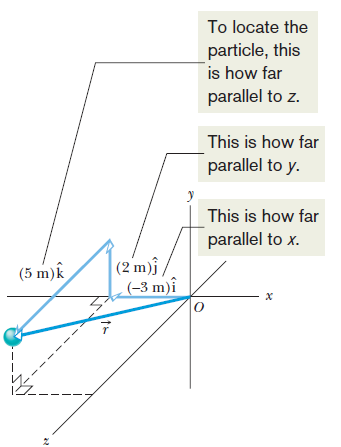
\includegraphics[width=0.9\linewidth]{position_vector}
		\end{column}
	\end{columns}
\end{frame}
%=======================================================================================================


%=======================================================================================================
\begin{frame}{The vector method}{Displacement vector}
	\begin{columns}
		\begin{column}{0.5\linewidth}
			As a particle moves, its position vector changes in such a way that the vector
			always extends to the particle from the reference point (the origin). If the position
			vector changes—say, from $\vec r_1$ to $\vec r_2$ during a certain time interval—then the
			particle’s \emph{displacement $\Delta \vec r$} during that time interval is
			\begin{equation*}
				\Delta  \vec r = \vec r_2 - \vec r_1.
			\end{equation*}
		\end{column}
		\begin{column}{0.5\linewidth}
			\includegraphics<1>[width=0.95\linewidth]{Displacement_vector_explanation}

			\includegraphics<2>[width=0.95\linewidth]{Displacement_vector}
		\end{column}
	\end{columns}
\end{frame}
%=======================================================================================================

%=======================================================================================================
\begin{frame}{The vector method}{Average Velocity and Instantaneous Velocity}
	\begin{columns}
		\begin{column}{0.5\linewidth}
			If a particle undergoes a displacement $\Delta\vec r$ in time interval $\Delta t$,
			its average velocity for that time interval is:
			\begin{equation*}
				\left\langle \vec v \right\rangle = \frac{\Delta \vec r}{\Delta t}
			\end{equation*}
		\end{column}
		\begin{column}{0.5\linewidth}
			When we speak of the velocity of a particle, we usually mean the particle’s
			instantaneous velocity at some instant.This $\vec v$ is the value $\left\langle \vec v \right\rangle$ that approaches in the limit as we shrink the time interval $t$ to 0 about that instant. Using the language of calculus, we may write as the derivative:
			\begin{equation*}
				\vec v = \frac{d \vec r}{d t}
			\end{equation*}
		\end{column}
	\end{columns}
\end{frame}
%=======================================================================================================


%=======================================================================================================
\begin{frame}{The coordinate method}{Components of Instantaneous Velocity}
	\begin{equation*}
		\vec v = \frac{d}{dt} (x\vec i + y\vec j + z\vec k) = \frac{dx}{dt}\vec i + \frac{dy}{dt}\vec j + \frac{dz}{dt}\vec k
	\end{equation*}
	So, the components of Instantaneous Velocity is:
	\begin{align*}
		v_x = 	\frac{dx}{dt} \\
		v_y = 	\frac{dy}{dt} \\
		v_z = 	\frac{dz}{dt}
	\end{align*}
\end{frame}
%=======================================================================================================


%=======================================================================================================
\begin{frame}{The vector method}{Direction of Instantaneous Velocity}

	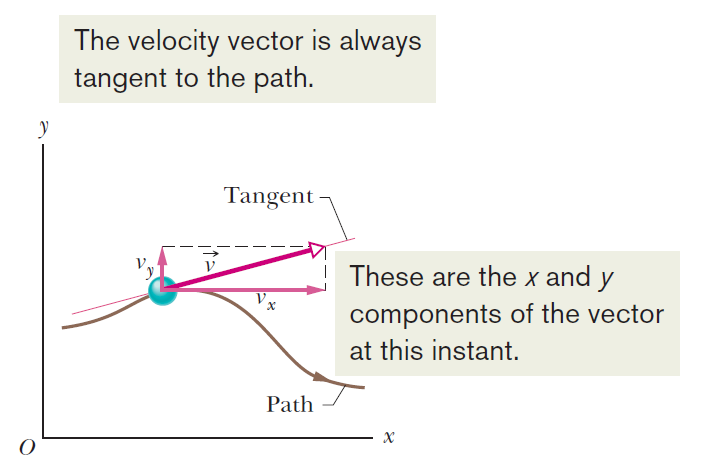
\includegraphics[width=0.85\linewidth]{Instantaneous_Velocity}
\end{frame}
%=======================================================================================================




%=======================================================================================================
\begin{frame}{The vector method}{Average Acceleration and Instantaneous Acceleration}
	\begin{columns}
		\begin{column}{0.5\linewidth}
			If a particle velocity changes from  $\vec v_1$ to $\vec v_2$ in time interval $\Delta t$,
			its average acceleration for that time interval is:
			\begin{equation*}
				\left\langle \vec a \right\rangle = \frac{\Delta \vec v}{\Delta t}
			\end{equation*}
		\end{column}
		\begin{column}{0.5\linewidth}
			When we speak of the acceleration of a particle, we usually mean the particle’s
			instantaneous acceleration at some instant. This $\vec a$ is the value $\left\langle \vec a \right\rangle$ that approaches in the limit as we shrink the time interval $t$ to 0 about that instant. Using the language of calculus, we may write as the derivative:
			\begin{equation*}
				\vec a = \frac{d \vec v}{d t}
			\end{equation*}
		\end{column}
	\end{columns}
\end{frame}
%=======================================================================================================


%=======================================================================================================
\begin{frame}{The coordinate method}{Components of Instantaneous Acceleration}
	\begin{equation*}
		\vec a = \frac{d}{dt} (v_x\vec i + v_y\vec j + v_z\vec k) = \frac{dv_x}{dt}\vec i + \frac{dv_y}{dt}\vec j + \frac{dv_z}{dt}\vec k
	\end{equation*}
	So, the components of Instantaneous Velocity is:
	\begin{align*}
		a_x = 	\frac{dv_x}{dt} \\
		a_y = 	\frac{dv_y}{dt} \\
		a_z = 	\frac{dv_z}{dt}
	\end{align*}
\end{frame}
%=======================================================================================================


%=======================================================================================================
\begin{frame}{The vector method}{Direction of Instantaneous Acceleration}

	\includegraphics[width=0.7\linewidth]{Instantaneous_Acceleration}
\end{frame}
%=======================================================================================================


%=======================================================================================================
\begin{frame}{Example}
	\begin{center}
		\includegraphics<1>[width=\linewidth]{Rabbit_1}
		\includegraphics<2>[width=\linewidth]{Rabbit_2}
		\includegraphics<3>[width=0.9\linewidth]{Rabbit_3}
		\includegraphics<4>[width=0.7\linewidth]{Rabbit_4}
	\end{center}
\end{frame}
%=======================================================================================================

%=======================================================================================================
\begin{frame}{The <<natural>> method}{Velocity of a point}
	\begin{overprint}
		\onslide<1>%
		This method is employed when the path of a point is known in advance. The location of a point $A$ is defined by the \emph{arc coordinate $s$}, that is, the distance from the chosen origin $O$ measured along the path.
		\onslide<2>%
		The velocity vector $\vec v$ of the point $A$ is oriented along a tangent to the path and therefore can be
		represented as follows:
		\begin{equation*}
			\vec v = v_\tau \vec \tau
		\end{equation*}
		where \emph{$v_\tau = \frac{ds}{dt}$} is the projection of the vector $\vec v$ on the direction of the vector $\vec\tau$, with $v_\tau$ being an algebraic quantity.
	\end{overprint}
	%---------------------------------------------------------
	\begin{overprint}
		\begin{center}
			\begin{tikzpicture}[scale=0.9]
				\draw [thick, red, tangent=0.3, decoration={markings,
							mark=at position 0.5 with \arrow{latex},
							mark=at position 0 with {
									\coordinate (O);
									\node[left, black] at (O) {$O$};
									\fill[black] circle [radius=2pt];
								},
							mark=at position 0.3 with {
									\coordinate (A);
									\node[below] at (A) {$A$};
									\fill[red] circle [radius=2pt];
								},
						},
					postaction=decorate] (0,0) coordinate[pos=0.4] (O) .. controls (1,3) and (3,1).. (4,4);
				\draw<2> [-latex, green!50!black, thick, use tangent] (0,0) -- (1.5,0) node[above] {$\vec v$};
				\draw<1-2> [-latex, blue, thick, use tangent] (0,0) -- (1,0) node[above] {$\vec\tau$};
				\node at ($(O)!0.5!(A)$) {$s$};
			\end{tikzpicture}
		\end{center}
	\end{overprint}
	%---------------------------------------------------------
\end{frame}
%=======================================================================================================

%=======================================================================================================
\begin{frame}{The <<natural>> method}{Acceleration of a point}
	If us differentiate Eq. \emph{$\vec v = v_\tau \vec \tau$} with respect to time we get an acceleration:
	\begin{equation*}
		\vec a = \frac{d\vec v}{dt} = \only<1->{\frac{dv_\tau}{dt}\vec\tau} + \only<2->{\frac{v^2}{\rho}\vec n}
	\end{equation*}

	\begin{columns}
		\begin{column}{0.4\linewidth}
			\begin{overprint}
				\begin{tikzpicture}
					\draw [thick, red, tangent=0.3, decoration={markings,
								mark=at position 0.5 with \arrow{latex},
								mark=at position 0 with {
										\coordinate (O);
										\node[left, black] at (O) {$O$};
										\fill[black] circle [radius=2pt];
									},
								mark=at position 0.3 with {
										\coordinate (A);
										\node[below] at (A) {$A$};
										\fill[red] circle [radius=2pt];
									},
							},
						postaction=decorate] (0,0) coordinate[pos=0.4] (O) .. controls (1,3) and (3,1).. (4,4);
					\draw<1-> [-latex, blue, thick, use tangent] (0,0) -- (2,0) coordinate (ET) node[above] {$\vec a_\tau$};
					\draw<1-> [-latex, blue, thick, use tangent] (0,0) -- (1,0) node[above] {$\vec\tau$};
					\draw<2-> [-latex, brown, thick, use tangent] (0,0) -- (-90:2) coordinate (EN) node[below] {$\vec a_n$}
					coordinate[pos=0.75] (Q)
					;
					\draw<2-> [-latex, brown, thick, use tangent] (0,0) -- (-90:1) node[below] {$\vec n$};
					\node at ($(O)!0.5!(A)$) {$s$};
					\draw<2>[dashed] (Q) circle (1.5);
					\draw<2>[-latex] (Q) -- node[below] {$\rho$} +(45:1.5);
					\draw<3>[dashed] (ET) -- ($(ET)!2cm!90:(A)$) coordinate (EA);
					\draw<3>[dashed] (EN) -- ($(EN)!2cm!-90:(A)$);
					\draw<3>[-latex, thick, green!50!black] (A) -- node[below] {$\vec a$} (EA);
				\end{tikzpicture}
			\end{overprint}
		\end{column}
		\begin{column}{0.6\linewidth}
			\begin{enumerate}
				\item<1-> Tangential acceleration \textcolor{blue}{$\vec a_\tau =  \frac{dv_\tau}{dt}\vec\tau$}
				\item<2-> Normal acceleration \textcolor{brown}{$\vec a_n =  \frac{v^2}{\rho}\vec n$}

				      {\small where $\rho$ of the corresponding circle as the radius of curvature of the path at
					      the same point.}

				\item<3-> Total acceleration \textcolor{green!50!black}{$\vec a =  \vec a_\tau + \vec a_n$}

				      {\small The magnitude of $\vec a$ is $a = \sqrt{a_\tau^2 + a_n^2}$ as shown in picture.}
			\end{enumerate}
		\end{column}
	\end{columns}

\end{frame}
%=======================================================================================================

\end{document}

